\documentclass[12pt,a4paper]{article}
\usepackage[utf8]{inputenc}
\usepackage[T1]{fontenc}
\usepackage{lmodern}
\usepackage{graphicx}
\usepackage{hyperref}
\usepackage{geometry}
\usepackage{setspace}
\usepackage{amsmath}
\geometry{a4paper, margin=1in}
\onehalfspacing

\title{Assignment 1: Classification and Prediction\\[1ex]
Machine Learning I\\
Course 2023-2024}
\author{Carlos Barboza --- 100472143\\
Lucas Monzón --- 100473232\\[2ex]
Departamento de Informática\\
Universidad Carlos III de Madrid}
\date{March 4, 2025}

\begin{document}

\maketitle
\thispagestyle{empty}
\newpage




\section*{Introduction}
In this project we apply machine learning techniques to the classical Snake game with the aim of both classifying the next move the snake should make and predicting future game scores. The overall objectives of the assignment are:
\begin{itemize}
    \item \textbf{Instances Collection:} Generate training and testing datasets by recording game states while playing manually.
    \item \textbf{Classification:} Build a classification model that predicts the snake's next move (North, South, East, or West) given a set of game state attributes.
    \item \textbf{Automatic Agent:} Integrate the chosen classification model with the Snake game to build an agent that plays automatically.
    \item \textbf{Prediction:} Develop a regression model that predicts the score in the next tick based on the current game state and the performed action.
\end{itemize}

The project follows an iterative approach, where initial experiments and feature extractions are refined based on the performance of both classification and regression models. In addition, techniques such as instance pruning are applied to improve data quality by removing undesirable actions taken during manual gameplay.

\newpage


\section{Phase 1: Instances Collection}

In this initial phase, the primary objective was to create a feature extraction method capable of generating ARFF files suitable for use in Weka. 
This involved modifying the existing function \texttt{printLineData()}, which we renamed to \texttt{get\_arff\_instance()} to fulfill the following three requirements:

\begin{enumerate}
    \item Generate ARFF files that Weka can successfully load by carefully defining attribute names, types, and structures.
    \item Ensure each instance in the ARFF file clearly describes the game state with relevant attributes, followed by the snake's executed action as the class attribute.
    \item Provide support to later include additional information related to future ticks, specifically the current and next tick scores, anticipating the regression tasks in subsequent phases.
\end{enumerate}

This process had to be done multiple times, as the initial feature set was refined based on the performance of the classification models in Phase 2.
Although multiple iterations of this function were created we will analyse only two of them.

The general structure and purpose of the function remains the same as in the previous assigments, but the attributes extracted and the way they are processed have been modified to better suit the classification (and later regression) task.

\subsection{Feature Extraction and ARFF Instance Generation}

In the implemented function, \texttt{get\_arff\_instance()}, collects key features describing the game state. The extracted attributes are:

\begin{itemize}
    \item \textbf{Snake and Food Positions}: Numeric coordinates (\texttt{head\_x, head\_y}) for the snake's head, and (\texttt{food\_x, food\_y}) for the food.

    \item \textbf{Directional Indicators}: Numeric attributes (\texttt{food\_left, food\_right, food\_up, food\_down}), indicating whether the food is positioned to the left, right, above, or below the snake’s head and the distance to the food in that direction (only positive values).

    \item \textbf{Adjacent Cell Occupancy Flags}: Four nominal (binary) attributes (\texttt{left\_occ, up\_occ, right\_occ, down\_occ}), indicating if the adjacent cells around the snake’s head are occupied by obstacles (body segments or walls).

    \item \textbf{Game Score and Manhattan Distance (Optional)}: Initially included, attributes such as the numeric game score and Manhattan distance between snake and food are computed, though these attributes were later excluded from the classification task and reserved for future phases involving prediction.

    \item \textbf{Distance to nearest obstacle (Only in the second iteration)}: The distance to the nearest obstacle in each of the four directions is calculated and included as numeric attributes in the ARFF file.

    \item \textbf{Class Attribute}: The snake’s executed action (\texttt{direction}) is stored as a nominal attribute with values \{\texttt{UP}, \texttt{DOWN}, \texttt{LEFT}, \texttt{RIGHT}\}.
\end{itemize}

We can find the code for the first iteration of the function in the Appendix~\autoref{sec:feature-extraction}.

This implementation ensures each instance is structured consistently, allowing seamless integration with Weka’s algorithms.

The original main set of features (without the distance to the nearest obstacle) was the one we settled on for the final classification model, as it provided the best balance between performance and complexity. 
Once we moved onto the third phase, when we integrated the model into the game, we found that the main problem was the snake enclosing itself, and the extended set of features (with the distance to the nearest obstacle) provided a better performance in this regard.
We will delve deeper into this in the next sections.


\subsection{ARFF File Generation}

For the header of the ARFF file, we made it that when the logs are flushed, the function checks if the file already exists. If it does not, it writes the header with the updated attributes. This ensures that the ARFF file is correctly formatted and ready for Weka processing.
And that we don't rewrite the header every time we flush the logs or start a new game.
We can find the code for the function in the Appendix~\autoref{sec:arff-logging}.

The header explicitly defines attribute names and types, matching the format expected by Weka, while the data section sequentially appends the collected instances.

\subsection{Preparing for Future Tick Information}

An important requirement was anticipating future regression tasks—specifically predicting the next tick’s score. The current design simplifies extending the instance format: the code structure readily accommodates adding further attributes (like next-tick scores). A future extension could easily append the score in the next tick as follows:

\begin{verbatim}
instance = f"{head_x},{head_y},{food_x},{food_y}," \
           f"{food_left},{food_up},{food_right},{food_down}," \
           f"{left_occ},{up_occ},{right_occ},{down_occ}," \
           f"{score},{next_tick_score},{direction}"
\end{verbatim}

This modification would directly enable supervised regression modeling in subsequent phases, demonstrating the function's flexibility.

\subsection{Data Collection}

For this phase, we divided it into two parts for each iteration of the function. 
In the first part, we let the $move_tutorial1$ function we implemented in the first assignment play the game, 
and we collected the instances generated by the function.
The instances were recorded in ARFF format, capturing the game state and the executed action.
This was done mostly in the early stages of the project, to quickly be able to test the classification performance for different feature sets.
As manually collecting instances is time-consuming.
Once we had a rough stimate of the performance of the different feature sets, we moved to the second part of the phase.
In the second part, we manually played the game, and we collected the instances generated by the function.
The collected data was then used to train and evaluate classification models in Phase 2.

\subsection{Summary:}
The feature extraction function was iteratively refined to capture relevant attributes for the classification task. 
We ended up with two different sets of features:

\textbf{Main Set:} Head and food positions, food direction indicators, adjacent cell occupancy flags, and the executed action.

\textbf{Extended Set:} The main set plus distances to the nearest obstacle in each cardinal direction.


\section{Phase 2: Classification}

Again, this phase was done intertwined with the first one, as we needed to test the performance of the different feature sets.
In this phase, we trained and evaluated classification models using the ARFF files generated in Phase 1. 
In this section we will mainly focus on the final results of the classification models, and the impact of the different feature sets on the performance of the models.
In this phase we won't delve into analysing the $Extended Set$ of features, as we will do that in the next phase, and will just focus on the $Main Set$ of features and different sets that didn't make the final cut.

\subsection{Data Pre-processing and Feature Selection}

The dataset used for this phase was generated during Phase 1. 
To ensure that only information available at decision time is used, we removed any attributes related to future ticks (e.g., the next tick's score). 
The final ARFF file used for training and testing has the following structure:

\begin{verbatim}
@relation snake_game-Weka

@attribute head_x numeric
@attribute head_y numeric
@attribute food_x numeric
@attribute food_y numeric
@attribute food_left numeric
@attribute food_up numeric
@attribute food_right numeric
@attribute food_down numeric
@attribute left_occ numeric
@attribute up_occ numeric
@attribute right_occ numeric
@attribute down_occ numeric
@attribute direction {UP,DOWN,LEFT,RIGHT}

@data
\end{verbatim}


The following pre-processing steps were carried out:
\begin{itemize}
    \item \textbf{Attribute Selection:} Only features available at the time of decision-making were retained (e.g., positions, relative food directions, and adjacent cell occupancy). Attributes related to future ticks were removed.
    \item \textbf{Filtering and Normalization:} Experiments were conducted to assess the impact of normalization, discretization, and balancing on classifier performance.
    \item \textbf{Instance Pruning:} To reduce noise from suboptimal moves, instances where we as a human player made clear mistakes were pruned out of the instace set.
\end{itemize}

We later performed an statistical analysis to determine the impact of the different pre-processing steps on the performance of the models and the game performance.

\subsection{Classification Experiments}
We experimented with several classification algorithms available in Weka, including:
\begin{itemize}
    \item \textbf{J48:} A decision tree algorithm.
    \item \textbf{NaiveBayes:} A probabilistic classifier based on Bayes' theorem.
    \item \textbf{k-Nearest Neighbors (k-NN):} A non-parametric classification method.
    \item \textbf{Random Forest:} An ensemble method based on multiple decision trees.
\end{itemize}

For each algorithm, models were trained on a training set (generated by manually playing the game) and evaluated on a separate testing set. The main evaluation metric was the percentage of correctly classified instances (CCI) for both training and testing datasets.

\subsection{Results and Analysis}
Table~\ref{tab:results} summarizes the key performance metrics for the classifiers we evaluated. The results are expressed in terms of the \textit{Correctly Classified Instances (CCI)} percentage for both training and testing datasets.

\begin{table}[ht]
\centering
\caption{Classification Performance Comparison with and without Instance Cleaning}
\label{tab:results}
\begin{tabular}{lcccc}
\hline
\textbf{Classifier} & \multicolumn{2}{c}{\textbf{Without Cleaning}} & \multicolumn{2}{c}{\textbf{With Cleaning}} \\ \hline
                    & \textbf{Training (\%)} & \textbf{Test (\%)} & \textbf{Training (\%)} & \textbf{Test (\%)} \\ \hline
J48                 & 90.15                       & 84.90                     & 93.81                       & 92.26                     \\
NaiveBayes          & 84.87                       & 86.81                     & 88.00                       & 87.07                     \\
5-NN                & 88.69                       & 83.55                     & 90.31                       & 85.25                     \\
10-NN               & 87.97                       & 85.94                     & 89.14                       & 86.12                    \\
Random Forest       & 99.90                       & 82.06                     & 99.93                       & 27.83                    \\ 
Logistic Function   & 87.02                       & 86.34                     & 89.86                       & 78.70                     \\\hline
\end{tabular}
\end{table}

Taking into account the set of possible actions, has a lenght of 4, the random selection of an action would have a CCI of 25\%.
These results indicate that while all classifiers perform reasonably well in both environoments (with and without instance cleaning)
we do see a significant improvement in the prediction accuracy when we clean the instances.
We will further analyse if this improvement does imply a better performance in the game in the next section.

We also must note that the Random Forest classifier has a significantly lower performance in the test set than in the training set, which indicates that the model is overfitting the training data.

All the files used for the experiments are available in the submission, as well as the resulting models.


\subsection{Phase 3: Binary Analysis}

Another test we tried to see if the performances changed was change the data type of the attributes from numeric to binary.
As we described before, we 8 attributes that correspond to the position of the food relative to the snake, and the occupancy of the adjacent cells.
Even if the data type of this attributes is numeric, they are binary in nature, as they can only take the values 0 or 1.
We decided to change the data type of this attributes to binary, and see if the performance of the models changed.
To do this we simply changed the data type of the attributes in the ARFF file from numeric to binary, and if at each instance the value was greater than 0 we set it to 1, and if it was 0 we set it to 0.
We then trained the models with this new data, and evaluated the performance of the models.
The results are shown in Table~\ref{tab:binary}.
\begin{table}[ht]
\centering
\caption{Classification Performance Comparison with Binary Attributes}
\label{tab:binary}
\begin{tabular}{lcc}
\hline
\textbf{Classifier} & \textbf{Training CCI (\%)} & \textbf{Testing CCI (\%)} \\ \hline
J48               & 93.80                       & 84.66                     \\
NaiveBayes        & 92.97                       & 84.43                     \\
5-NN              & 93.92                       & 84.34                     \\
10-NN             & 93.96                       & 84.51                     \\
Random Forest     & 99.92                       & 83.76                     \\ 
Logistic Function & 93.87                       & 84.77                     \\\hline
\end{tabular}
\end{table}


In this new results we see that in the test set the performance of the models is very similar (if not slightly worse) than the performance of the models with the numeric attributes.
The biggest difference is in the Random Forest classifier, which has a way better performance in the test set with the binary attributes, 
indicating that the model is not overfitting the training data as much as with the numeric attributes.
This is a very interesting result, as it shows that the binary attributes are more informative than the numeric attributes, and that the models can learn better from them.
Also another key difference is that the J48 has a worse performance in the test set with the binary attributes. 

It is important to note that the actual final metric we will use is the performance of this models in the game, and not the performance in the classification task.
We will further analyse this in the next section.




\subsection{Discussion}
The experiments highlighted several real-world observations:
\begin{itemize}
    \item \textbf{Impact of Instance Pruning:} Removing noisy instances markedly improved test accuracy. This cleaning reduced overfitting, particularly evident in classifiers such as Random Forest.
    \item \textbf{Numeric vs. Binary Attributes:} Switching from numeric to binary attributes had mixed effects. While most classifiers maintained similar performance, the binary representation notably reduced the overfitting seen with Random Forest, even though models like J48 experienced a slight drop in test accuracy.
    \item \textbf{Importance of Data Pre-processing:} The results reinforced that careful feature selection, normalization, and instance pruning are crucial in balancing model complexity with generalization to unseen data.
\end{itemize}

Overall, these observations directly influenced our final model selection and integration strategy for the automatic agent.


\section{Phase 3: Building an Automatic Agent}

In this phase, our objective is to integrate the previously generated classification model with the Snake game so that the agent can autonomously decide its next move based on the current game state. This automatic agent replaces manual control (via keyboard input) and improves upon the baseline heuristic agent developed in Tutorial 1.

\subsection{Integration with Weka}

To achieve this, we use the \texttt{wekaI.py} interface. The following steps were taken to connect the game with the machine learning model:

\begin{enumerate}
    \item \textbf{Weka Environment Setup:}
    We ensured that a compatible Java compiler and interpreter were installed, along with the required Python packages \texttt{javabridge} and \texttt{python-weka-wrapper3}. At the top of our code, we import the \texttt{Weka} class:
    \begin{verbatim}
from wekaI import Weka
    \end{verbatim}

    \item \textbf{Launching the Java Virtual Machine:}
    An instance of the \texttt{Weka} class is created and the Java Virtual Machine is started during game initialization:
    \begin{verbatim}
weka = Weka()
weka.start_jvm()
    \end{verbatim}

    \item \textbf{Model Prediction:}
    In each iteration of the game loop, the current state of the game is captured via the \texttt{get\_instance\_attributes(game)} function. This feature vector is then passed to the \texttt{weka.predict()} method along with the model file and the ARFF file used during training. For example:
    \begin{verbatim}
x = get_instance_attributes(game)
weka_direction = weka.predict("./Models/j48.model", x, "./Arffs/bina_pruned2.arff")
game.direction = weka_direction
    \end{verbatim}
    The predicted direction is then assigned to \texttt{game.direction}, which dictates the snake's next move.
\end{enumerate}

\subsection{Agent Behavior and Performance Comparison}

The automatic agent operates by continuously:
\begin{itemize}
    \item Capturing the current game state.
    \item Using the machine learning model to predict the optimal move.
    \item Executing the predicted move in real time.
\end{itemize}

For this initial implementation we ran the best performing model from the classification experiments in Phase 2,
specifically with the cleaned instances and the binary attributes.

We can see their base performance in the following image:

\begin{figure}[ht]
    \centering
    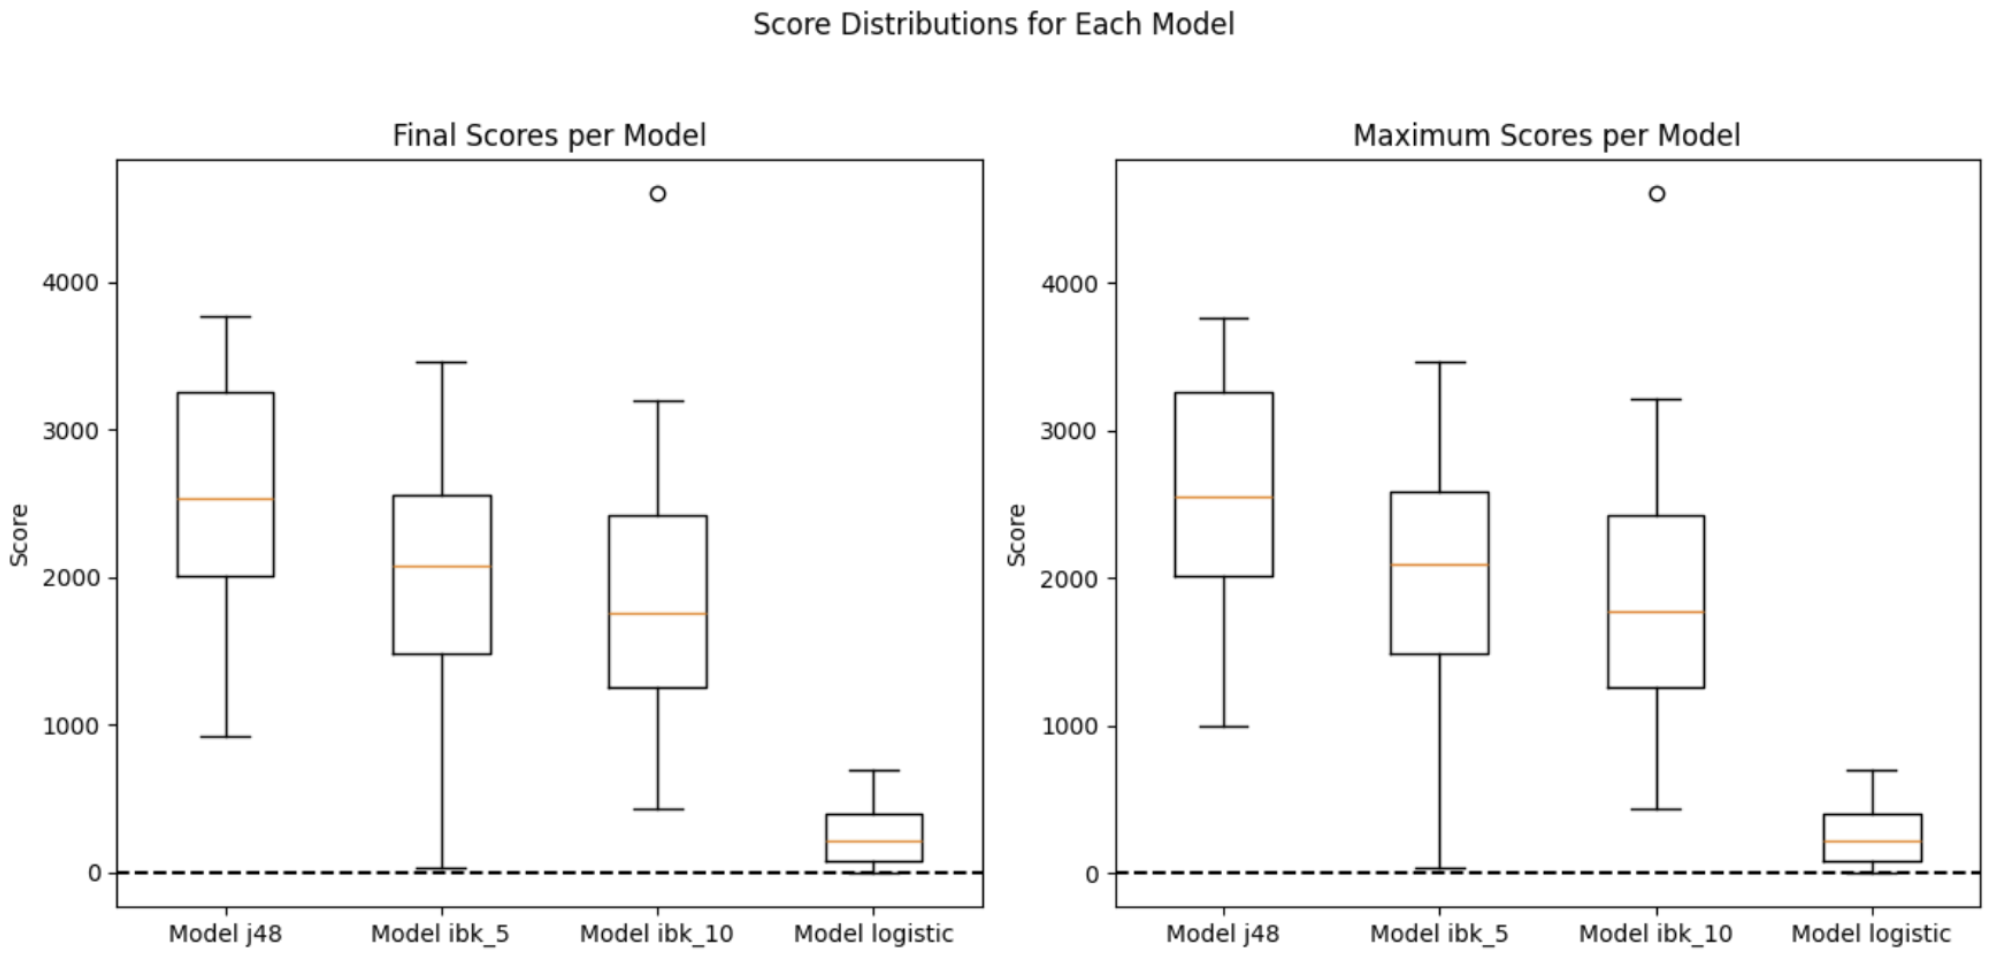
\includegraphics[width=0.9\textwidth]{./images/main_models.png} %%% Change this
    \caption{Game Performance of the Automatic Agent}
    \label{fig:game}
\end{figure}

As we can see even if most models have a similar performance in the classification task, the performance in the game is very different.
specifically the Random Forest model has a very poor performance in the game, even if it has a good performance in the classification task.
This is a very interesting result, as it shows that the performance in the classification task is not a good indicator of the performance in the game.
Here the K-NN with 10 neighbors model has the best performance in the game (if slightly), even if it has a worse performance in the classification task.

All this test were done using the binary attributes, as they had a better performance in the classification task, and we wanted to see if this translated to a better performance in the game.

\subsection{Model Comparison and Analysis}

As discussed previously once we saw the models real performance in the game, 
we noticed that it mostly failed when the snake enclosed itself, and the main problem was that the snake was not able to escape from this situations.
This is a very interesting result, as it shows that the models are not able to learn the concept of being enclosed, 
or in general: the model is not aware of the "big picture" of the game.

This could also easily be deduced, as the models are only trained with the current state of the game, and only on a few parameters of it.
If we were to include more parameters, as the exact position of the snake, or the position of the walls, the model could learn to avoid enclosing itself,
howerver this would make the model more complex, possible leading to overfitting, and would make the model harder to train.

This could be a very interesting point to explore in future work, as it could lead to a more robust model, that could be able to play the game in a more human-like way.
However for this task in particular a reinforcment learning approach could be more suitable, as it would allow the model to learn from the consequences of its actions, and not only from the current state of the game.

We deduced that maybe if we gave it more informaiton about it's surroundings, it could learn to avoid enclosing itself.
We settled on the second model we implemented in the first phase. 
We ran some tests with this model, and that even if it had a similar performance, it was actually slightly worse than the best model we had.
Maybe because we aren't actually giving the model the information it needs to avoid enclosing itself, or maybe because the model is too simple to learn this concept.
Even if it's a simple model, we increase slightly the complexity, making it perform slightly worse than out previous model.

\begin{figure}[ht]
    \centering
    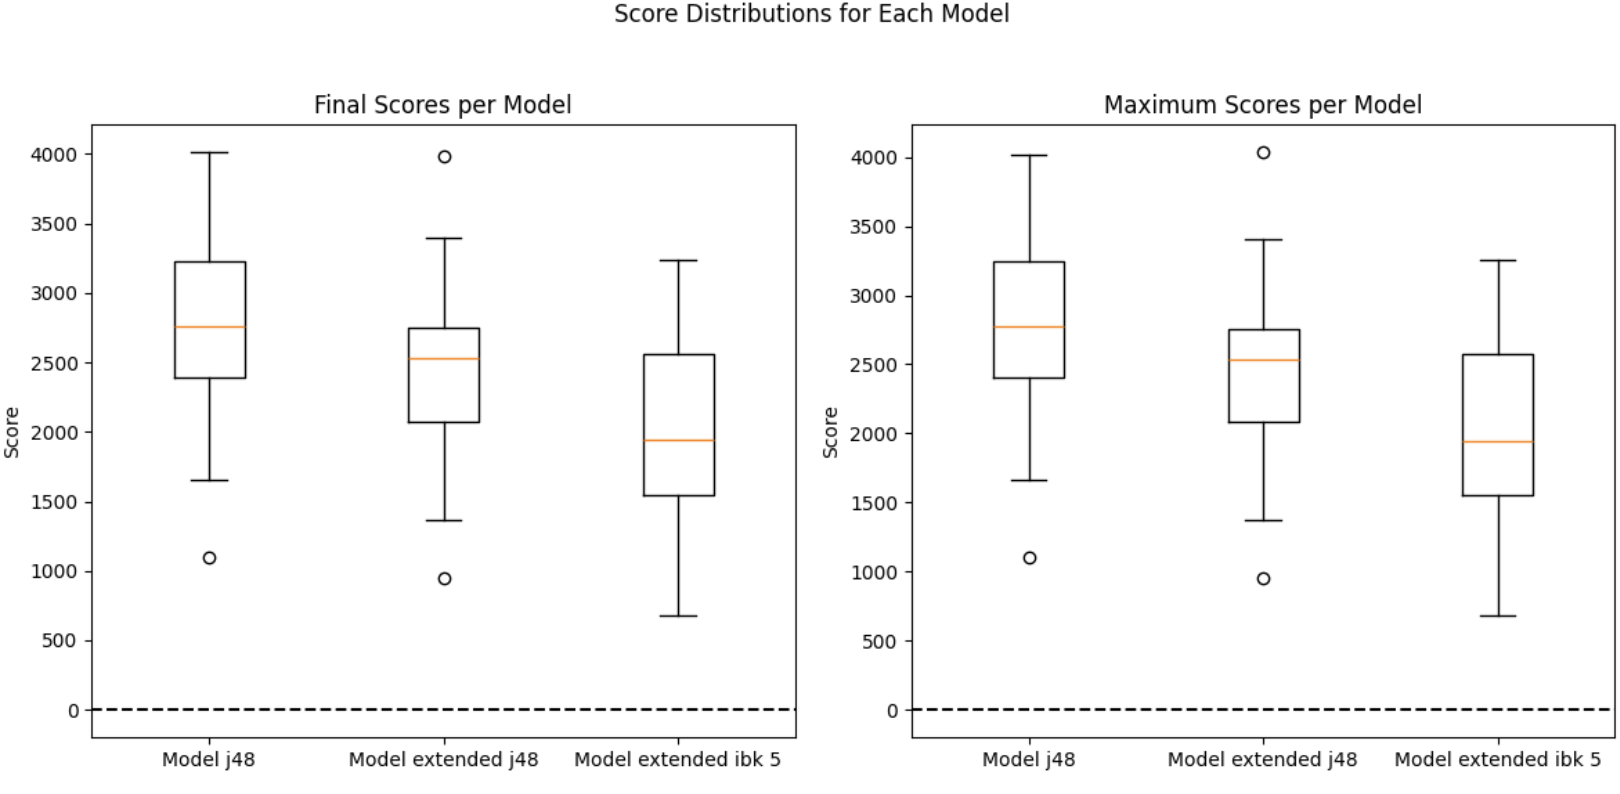
\includegraphics[width=0.9\textwidth]{./images/extended.png} %%% Change this
    \caption{Game Performance of the Automatic Agent vs the Heuristic Agent}
    \label{fig:game}
\end{figure}


\subsection{Model comparaison against the heuristic agent}

We also compared the performance of the automatic agent against the heuristic agent we implemented in the first tutorial.
We can find the results in the following image:

\begin{figure}[ht]
    \centering
    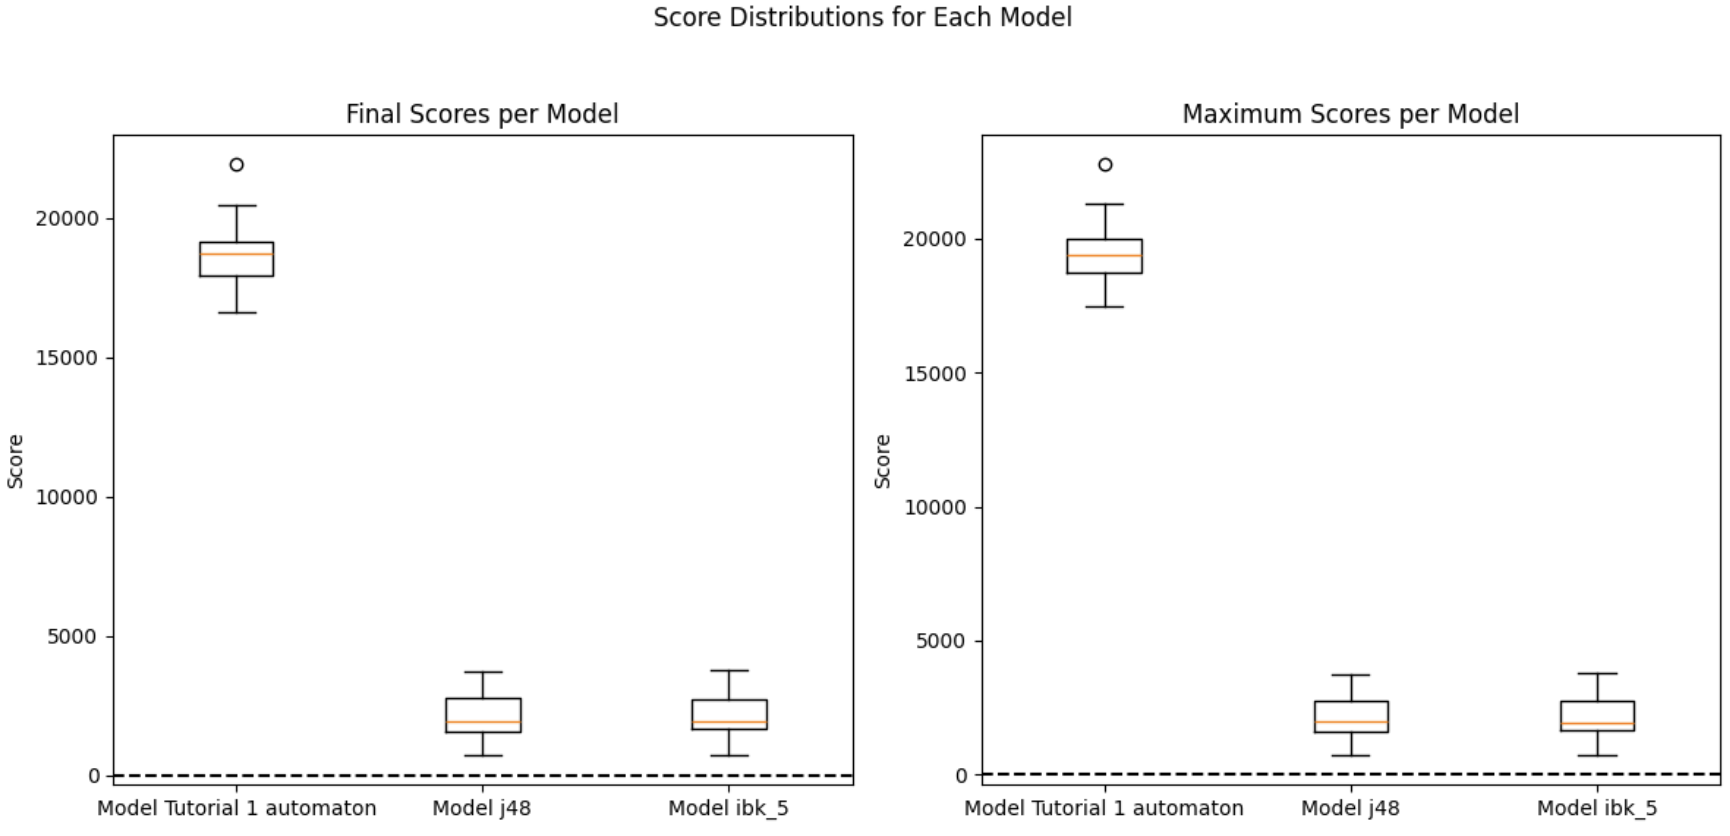
\includegraphics[width=0.9\textwidth]{./images/heuristic.png} %%% Change this
    \caption{Game Performance of the Automatic Agent vs the Heuristic Agent}
    \label{fig:game}
\end{figure}

As we can see the automatic agent has a way worse performance than the heuristic agent. 
This is mainly as we took great care in the heuristic agent to avoid the snake enclosing itself.

As they both present a similar performance if we were to not increase the lenght of the snake. 
However as the lenght of the body increases where the heuristic agent can keep track of it, 
mainly by analysing at each step if taking any action would lead to the snake enclosing itself.

Another key difference is the speed of the agents, as the heuristic agent is way faster than the automatic agent.
As the test for both agents took around the same time, whereas the heuristica agent was able to have games 10 times longers


\subsection{Human vs. Automatic Agent Training Performance}

We also compared the performance of our models if they were trained by a human player or by the automatic agent.
All the following results were obtained using the binary attributes, and the cleaned instances.

\begin{figure}[ht]
    \centering
    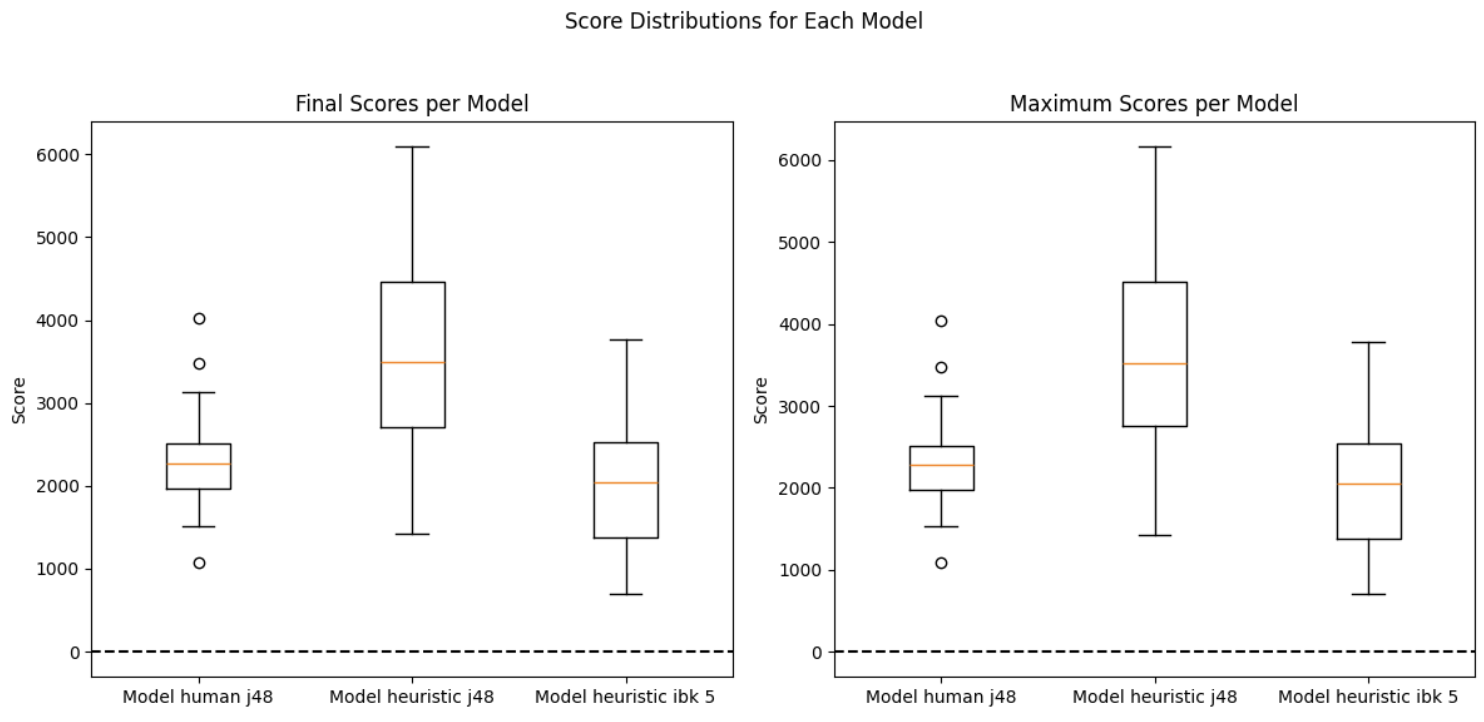
\includegraphics[width=0.9\textwidth]{./images/heuristic_training.png} %%% Change this
    \caption{Game Performance of the Human Agent vs the Automatic Agent}
    \label{fig:game}
\end{figure}

We can clearly see that the models trained by the heuristic agent have a better performance than the models trained by the automatic agent.
this will be further explored in the questions section.



\section{Phase 4: Prediction}
\subsection{Regression Model for Score Prediction}
Beyond action classification, our assignment also required us to build a regression model to predict the game score in the next tick. The regression model uses similar state attributes along with the performed action as inputs, and the target variable is the score at the following tick.

\subsection{Experimental Setup and Results}
We experimented with at least two regression algorithms, such as linear regression and M5P (model trees), to determine which could better predict the incremental score changes. Pre-processing steps similar to those in Phase 2 were applied. The evaluation metrics included mean absolute error and root mean squared error. A detailed analysis of the performance across different algorithms helped us to understand the sensitivity of the score prediction task and guided us in selecting the final model.

\section{Questions}
\subsection*{1. Difference between Human-Controlled and Automatic Agents}
The primary difference lies in the variability and suboptimality of human decisions. 
Human-controlled instances often include mistakes and inconsistent strategies, whereas an automatic agent, once properly trained, can consistently apply the learned policy. 
This leads to differences in both classification accuracy and overall game performance.

Even if we removed most of the mistakes from the instances, the human player still makes suboptimal decisions,
and has a very simplistic strategy, mainly going directly to the food, and only changing direction when it is blocked.
However as the heuristic agent uses Hilber curves to decrease the changes of enclosing itself, it has a more complex strategy, and is able to play the game for longer periods of time.
The model could (and did) pick up some of this strategy, even if imperfectly, improving the performance of the automatic agent.



\subsection*{2. Transforming Regression to Classification}
To transform the regression task (predicting the score) into a classification task, the continuous score values can be discretized into bins or ranges. 
For example, one could classify the expected score change as \texttt{high increase}, \texttt{moderate increase} or \texttt{decrease}. 
Even if in reality the score can only decrease by one or increase by 100, 
we also introduce the \texttt{moderate increase} class, to let the model be able to 
Such discretization could have practical applications in designing adaptive difficulty or reward mechanisms in games.

\subsection*{3. Advantages of Predicting Score over Classifying Action}
Predicting the score provides a quantitative measure of the agent’s performance and allows for the evaluation of long-term strategies. In contrast, classifying the action only addresses immediate decisions. A regression model for score prediction can help refine the agent’s overall strategy by correlating certain moves with higher future rewards.

\subsection*{4. Incorporating an Attribute for Score Drop}
Including an attribute that indicates whether the current score most likely  wouldn't improve performance, mainly becuase of two reasons:
\begin{itemize}
    \item \textbf{Complexity:} Adding a new attribute could increase the model's complexity and the dimensionality of the feature space, potentially leading to overfitting.
    \item \textbf{Redundancy:} When traing the model we would have much more instances where the score would drop, as it drops by one for each step the snake doesn't eat the food. While eating the food is a "rare" event.
\end{itemize}
As almost all the instances would have a score drop,
the distribution of the classes would be almost uniform, inside this attribute, not really adding any information to the model.





\section{Conclusions}
In this assignment, we successfully applied machine learning techniques to both classify the next action in a Snake game and predict future scores. Our iterative process involved careful instance collection, data pre-processing (including instance pruning), and the integration of Weka models into the game environment. While the automatic agent shows promising improvements over manual control, further work is required to handle more dynamic and complex in-game situations. The experiments conducted provided valuable insights into the advantages and challenges of applying machine learning to real-time decision-making in games.

\vspace{1em}
\noindent\textbf{Future Work:} Future research could explore more advanced reinforcement learning techniques, incorporate additional sensory attributes, and experiment with ensemble methods for both classification and regression tasks.


\newpage
\section{Appendix}

\subsection{Code Listings}

You can find the full code for the project in the following link:
\href{https://github.com/carlos1302-ai/projec1_ml}{Project Code Repository}


\subsubsection{Feature Extraction Function}
\label{sec:feature-extraction}

Below is the Python implementation of the \texttt{get\_arff\_instance()} function used for feature extraction:

\begin{verbatim}
    def get_arff_instance(game):
    """
    Returns a string in ARFF format representing the current game state,
    including distances to the nearest obstacle in the four cardinal directions.
    """
    head_x, head_y = game.snake_pos
    food_x, food_y = game.food_pos

    # Compute food direction indicators (binary)
    food_left  = 1 if food_x < head_x else 0
    food_right = 1 if food_x > head_x else 0
    food_up    = 1 if food_y < head_y else 0
    food_down  = 1 if food_y > head_y else 0

    # Check occupancy for adjacent cells
    def occupied(cell):
        if cell[0] < 0 or cell[0] >= FRAME_SIZE_X or cell[1] < 0 or cell[1] >= FRAME_SIZE_Y:
            return 1
        return 1 if (cell in game.snake_body and cell != game.snake_body[-1]) else 0

    left_cell  = [head_x - 10, head_y]
    up_cell    = [head_x, head_y - 10]
    right_cell = [head_x + 10, head_y]
    down_cell  = [head_x, head_y + 10]

    left_occ  = occupied(left_cell)
    up_occ    = occupied(up_cell)
    right_occ = occupied(right_cell)
    down_occ  = occupied(down_cell)

    direction = game.direction
    score = game.score
    manhattan_distance = abs(head_x - food_x) + abs(head_y - food_y)

    next_head = [head_x, head_y]
    if direction == "UP":
        next_head[1] -= 10
    elif direction == "DOWN":
        next_head[1] += 10
    elif direction == "LEFT":
        next_head[0] -= 10
    elif direction == "RIGHT":
        next_head[0] += 10

    if next_head == game.food_pos:
        next_score = score + 100
    else:
        next_score = score - 1

    # New helper: compute distance to obstacle in a given direction
    def distance_in_direction(dx, dy):
        distance = 0
        current = [head_x, head_y]
        while True:
            current[0] += dx
            current[1] += dy
            distance += 10  # step size
            # Check for wall collision
            if current[0] < 0 or current[0] >= FRAME_SIZE_X or current[1] < 0 or current[1] >= FRAME_SIZE_Y:
                break
            # Check for collision with snake body (exclude tail, similar to occupied())
            if current in game.snake_body and current != game.snake_body[-1]:
                break
        return distance

    # Compute distances in each cardinal direction
    dist_left = distance_in_direction(-10, 0)
    dist_up = distance_in_direction(0, -10)
    dist_right = distance_in_direction(10, 0)
    dist_down = distance_in_direction(0, 10)

    # Append the new obstacle distance parameters to the ARFF instance.
    instance = f"{head_x},{head_y},{food_x},{food_y}," \
               f"{food_left},{food_up},{food_right},{food_down}," \
               f"{left_occ},{up_occ},{right_occ},{down_occ}," \
               f"{score},{next_score},{manhattan_distance}," \
               f"{dist_left},{dist_up},{dist_right},{dist_down},"\ # Comment this 
                #line to return the first iteration
                f"{direction}"
    return instance
\end{verbatim}

\subsubsection{ARFF File Logging Function}
\label{sec:arff-logging}
The following code snippet demonstrates the implementation of the \texttt{flush\_logs()} function for ARFF file generation:

\begin{verbatim}
    def flush_logs():
    """
    Writes buffered ARFF log entries to 'game_log.arff'.
    If the file is new, writes the header with the updated attributes.
    """
    filename = "game_log.arff"
    if not os.path.isfile(filename):
        header = """@relation snake_game

@attribute head_x numeric
@attribute head_y numeric
@attribute food_x numeric
@attribute food_y numeric
@attribute food_left numeric
@attribute food_up numeric
@attribute food_right numeric
@attribute food_down numeric
@attribute left_occ numeric
@attribute up_occ numeric
@attribute right_occ numeric
@attribute down_occ numeric
@attribute score numeric
@attribute next_score numeric
@attribute manhattan_distance numeric
@attribute dist_left numeric    # Comment this lines to return the first iteration
@attribute dist_up numeric      #
@attribute dist_right numeric   #
@attribute dist_down numeric    # End of comment
@attribute direction {UP,DOWN,LEFT,RIGHT}
@data
"""
        with open(filename, "w") as f:
            f.write(header)
    if log_buffer:
        with open(filename, "a") as f:
            f.write("\n".join(log_buffer) + "\n")
        log_buffer.clear()

\end{verbatim}



\end{document}